\chapter{Q-larning algoritmus}

Q-learning algoritmus je definovaný pre časovo diskrétne systémy.
Agent ktorý prechádza stavový priestor vykonaním niektorej z vopred daných
akcií získava za tieto prechody odmeny. Cieľom algoritmu je ohodnotiť všetky akcie
v jednotlivých stavoch, tak aby bol dosiahnutý ustálený stav a v každom stave
bolo možno vybrať akciu prinášajúcu najväčšiu odmenu, v zmysle
s \ref{eq:q_quality}.


\section{Definícia algoritmu}

Autorom Q-learning algoritmu je Christopher J.C.H. Watkins, v roku 1992 publikoval
článok kde tento algoritmus predstavil \cite{bib:q_learning_watkins} a niekoľko ďalších,
jednoduchých vysvetlení tohto algoritmu je možné nájsť v \cite{bib:q_tutorial_01} alebo
\cite{bib:q_tutorial_02}. Dôkazy o konvergencií k otimálnemu riešeniu (v zmysle
s \ref{eq:q_quality}) sú k dispozícií \cite{bib:q_proof_01}, \cite{bib:q_proof_02},
\cite{bib:q_proof_03}, \cite{bib:q_proof_04}.

Daná je množina stavov $\mathbb{S}$ a akcií $\mathbb{A}$, kde
 $\mathbb{S} \in \mathbb{R}^{n_s}$ a $\mathbb{A} \in \mathbb{R}^{n_a}$, kde
$n_s$ a  $n_a$ sú počty prvkov stavového vektora a vektora akcií.

Existuje prechodová funkcia
\begin{align}
        s(n+1) = \lambda(s(n), a(n))
\end{align}

zo stavu $s(n) \in \mathbb{S}$ použitím akcie $a(n) \in \mathbb{A}$, táto funkcia je ale algoritmu neznáma,
v reálnom prostredí je jej výsledok obvykle stochastický.

Ďalej je daná odmeňovacia funkcia $R(s(n),a(n))$, ktorá vyjadruje okamžité ohodnotenie konania
agenta v $s(n)$ a $a(n)$. V reálnych aplikáciach táto funkcia nadobúda takmer v každom
$s(n)$ a $a(n)$ hodnotu $0$. Pre správnu funkciu algoritmu, musí byť aspoň jedna hodnota
nenulová - napr. ohodnotenie dosiahnutia cieľového stavu (samotná existencia cieľového
stavu však pre algoritmus nie je potrebná).

Funkcia ohodnotení je definovaná ako

\begin{equation}
Q_{n}(s(n),a(n)) = R(s(n),a(n)) + \gamma \max_{a(n-1) \in \mathbb{A}} Q_{n-1}(s(n-1), a(n-1))
\label{eq:q_learning}
\end{equation}

\begin{itemize}
 \item $R(s(n),a(n))$ je odmeňovacia funkcia
 \item $Q_{n-1}(s(n-1),a(n-1))$ je funkcia ohodnotení v stave $s(n-1)$ pre akciu $a(n-1)$
 \item $\gamma$ je odmeňovacia konštanta a platí $\gamma \in (0, 1)$.
\end{itemize}

Funkcia $\ref{eq:q_learning}$ definuje ohodnotenie akcií vo všetkých stavoch t.j.
agent ktorý sa dostal do stavu $s(n)$ vykonaním akcie $a(n)$ zo stavu
$s(n-1)$ získal odmenu $R(s(n),a(n))$ a zlomok najväčšieho možného ohodnotenia ktoré
mohol získať dostaním sa do stavu $s(n-1)$, situáciu ilustruje obrázok \ref{img:q_learning}.


\begin{figure}[!htb]
\center
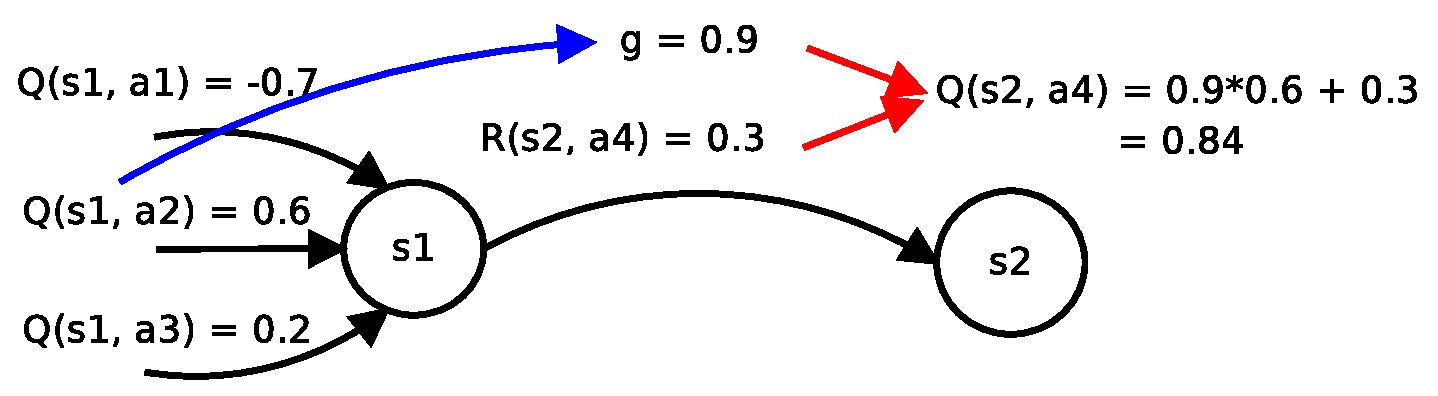
\includegraphics[scale=.6]{../diagrams/q_learning_detail.eps}
\caption{Ilustrácia funkcie ohodnotení, pre $\gamma = 0.9$}
\label{img:q_learning}
\end{figure}

Je potrebné poznamenať, ža práve časť $\max_{a(n-1) \in \mathbb{A}} Q_{n-1}(s(n-1), a(n-1)$
zabezpečuje nezávislosť konvergencie k optimu bez ohľadu voľby stratégie výberu akcie -
postačuje, aby každá akcia, v každom stave mala nenulovú pravdepodobnosť vykonania.
Určitým variantom, je algoritmus SARSA \cite{bib:sarsa}

\begin{align}
Q_{n}(s(n),a(n)) &= \nonumber \\
 (1-&\alpha)Q_{n-1}(s(n),a(n)) + \nonumber  \\
&\alpha(R(s(n),a(n)) + \gamma Q_{n-1}(s(n-1), a(n-1)))
\label{eq:sarsa}
\end{align}

kde $\alpha \in (0, 1)$, hodnota $Q_{n}(s(n),a(n))$ sa  teda ustáli na strednej hodnote,
a závisí na stratégie výberu akcií. Q-learning teda vychádza z toho, čo najlepšie sa mohlo stať
a SARSA z toho čo sa naozaj stalo.


Nasledujúce obrázky ilustrujú beh algoritmu pre systém so 6 stavmi pre $\gamma = 0.8$.
Na začiatku nie sú známe ani samotné prechody medzi stavmi (Obr. $\ref{img:q_learning_1}$), bol definovaný
1 cieľový stav $S5$, agent začína v stave $S0$ (môže však v ľubovolnom inom).
Ďalej sa pre jednoduchosť predpokladá že

\begin{equation}
R(s(n), a(n)) =
\left\{
	\begin{array}{ll}
		1  & ak \ s(n) = $S5$ \\
    -0.5  & ak \ s(n) = $S4$ \ \wedge \ $a(n) = Ay$  \\
		0 & inak
	\end{array}
\right.
\label{eq:r_func_simple}
\end{equation}

t.j. odmeňovacia funkcia nadobúda hodnotu $1$ len ak sa agent dostal do stavu
$S5$ a pre ilustráciu je definovaná aj jedna záporná odmena pri prechode z $S4$ do
$S3$ akciou $Ay$.

\begin{figure}[!htb]
\center
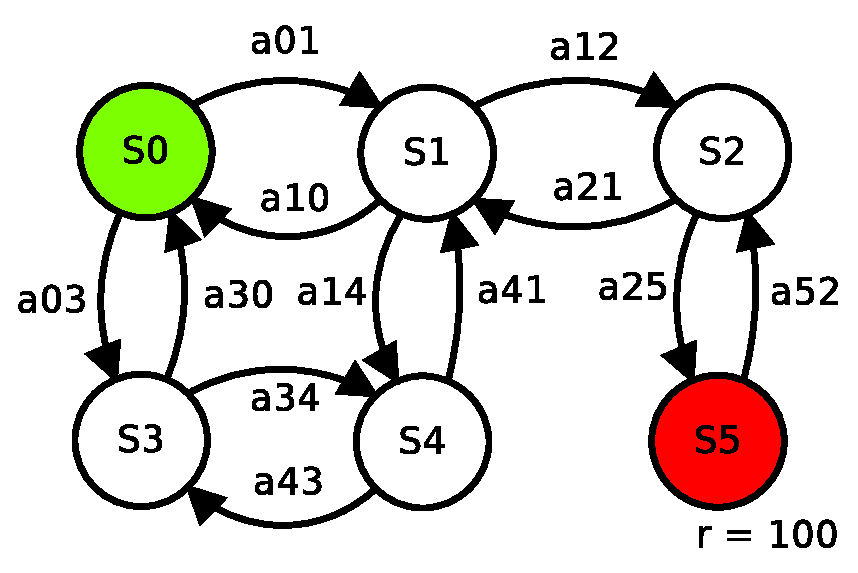
\includegraphics[scale=.6]{../diagrams/q_learning_table_01.eps}
\caption{Inicializácia}
\label{img:q_learning_1}
\end{figure}

Agent v každom stave náhodne vyberá akcie (na výbere nezáleží, dôležité je aby
každá akcia mala nenulovú pravdepodobnoť výberu, a rovnako bola nenulová
prevdepodobnosť dosiahnutia ľubovolného stavu). Obrázky Obr. \ref{img:q_learning_2}
a Obr. \ref{img:q_learning_3} ilustrujú jednu z možných ciest.


\begin{figure}[!htb]
\center
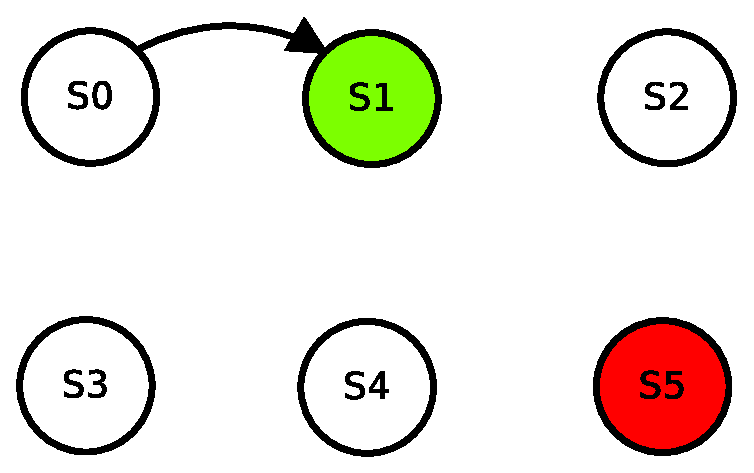
\includegraphics[scale=.6]{../diagrams/q_learning_table_02.eps}
\caption{Prechod do stavu S1}
\label{img:q_learning_2}
\end{figure}

\begin{figure}[!htb]
\center
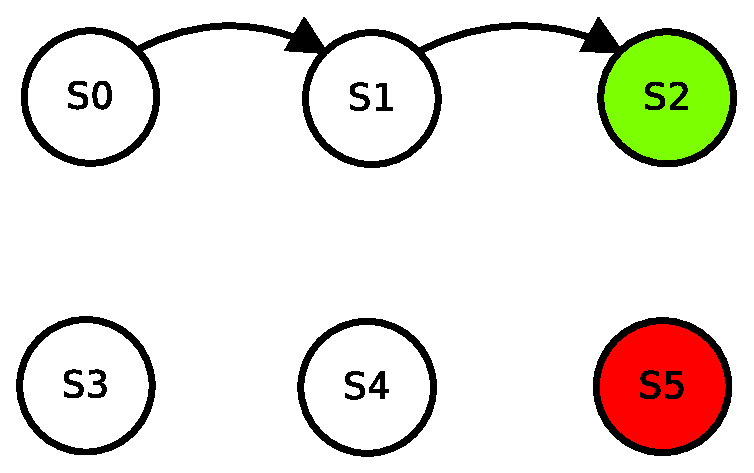
\includegraphics[scale=.6]{../diagrams/q_learning_table_03.eps}
\caption{Prechod do stavu S2}
\label{img:q_learning_3}
\end{figure}

Po dosiahnutí cieľového stavu Obr. \ref{img:q_learning_4} je na základe \ref{eq:r_func_simple}
možné spočítať podľa \ref{eq:q_learning} ohodnotenia doteraz vykonaných akcií -
agent získal nenulovú odmenu $R(s_5, a_x) = 1$ (kde $a_x$ značí ľubovolnú akciu),
ktorú rekurentne spočíta pre všetky doteraz vykonané akcie.

Pre zjednodušenú variantu \ref{eq:q_learning} by bolo možné pamätať si len jeden
predošlý stav a nepostupovať v ohodnocovaní rekuretne. V praktickej aplikácií
je potrebné obmedziť hĺbku rekurzie, a pamätať si len posledných $P$ stavov a vnich
urobených rozhodnutiach. V tomto jedńoduchom príklade však nie sú nutné tieto obmedzenia, je teda
možné pamätať si celú cestu.

\begin{figure}[!htb]
\center
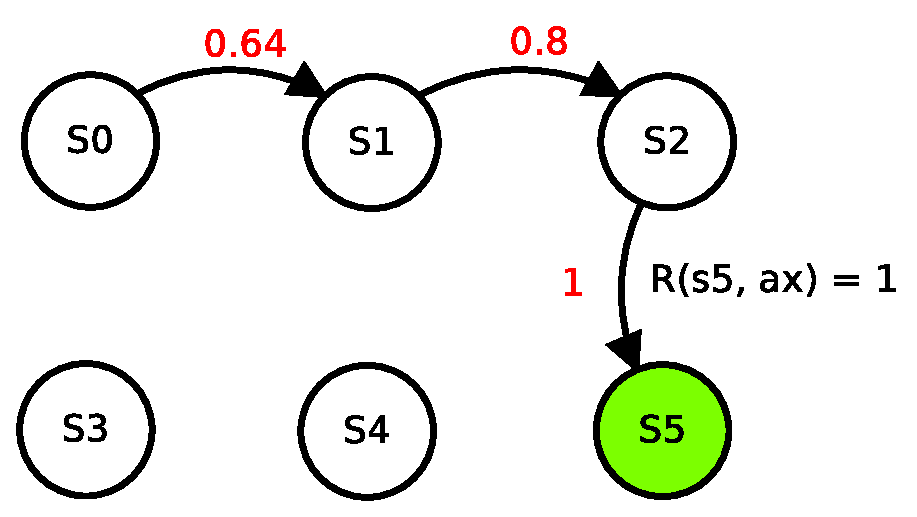
\includegraphics[scale=.6]{../diagrams/q_learning_table_04.eps}
\caption{Prechod do stavu S3}
\label{img:q_learning_4}
\end{figure}

Agent môže pokračovať v ceste ďalej, napr. späť \ref{img:q_learning_5} a pribežne
počítať ohodnotenia. Prechod z $s_5$ do $s_2$ je ohodnotený ako $0.8$ - vybralo sa najlepšie
možné ohodnotenie ako sa dostať do $s_5$ ($1$) násobené $\gamma$, $R(s_2, a_x) = 0$
(podľa \ref{eq:r_func_simple}).


\begin{figure}[!htb]
\center
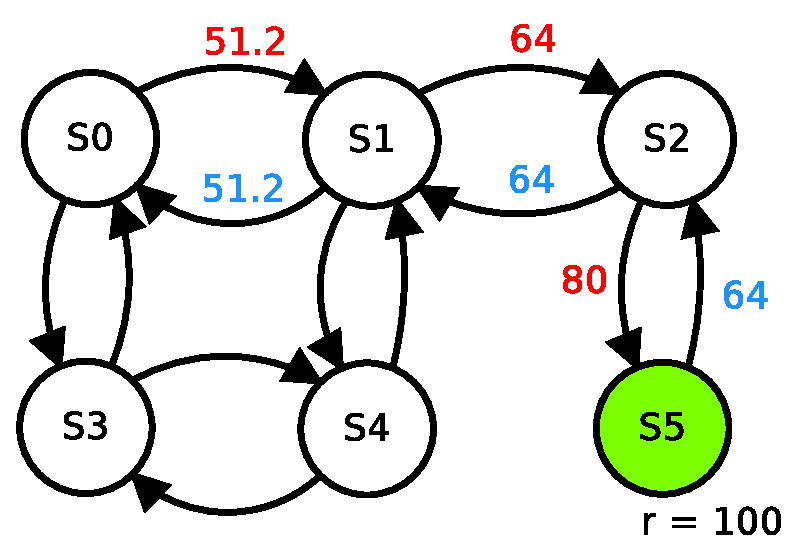
\includegraphics[scale=.6]{../diagrams/q_learning_table_05.eps}
\caption{Ďalšie prechody agenta}
\label{img:q_learning_5}
\end{figure}

Po prejdení celého grafu, kedy agent vykonal všetky možné akcie dosiahne
funkcia $Q(s(n), a(n))$ konečný, ustálený stav Obr. \ref{img:q_learning_6}, teda

\begin{equation}
\forall s(n),\ \forall a(n),\forall \epsilon > 0 \  \exists Q_{n} : \mid Q_{n}(s(n), a(n)) - Q_{n-1}(s(n), a(n)) \mid < \epsilon
\label{eq:q_learning_finish}
\end{equation}

hodnoty Q-funkcie sa teda pri pevne danom $R(s(n), a(n))$ už nemenia.


\begin{figure}[!htb]
\center
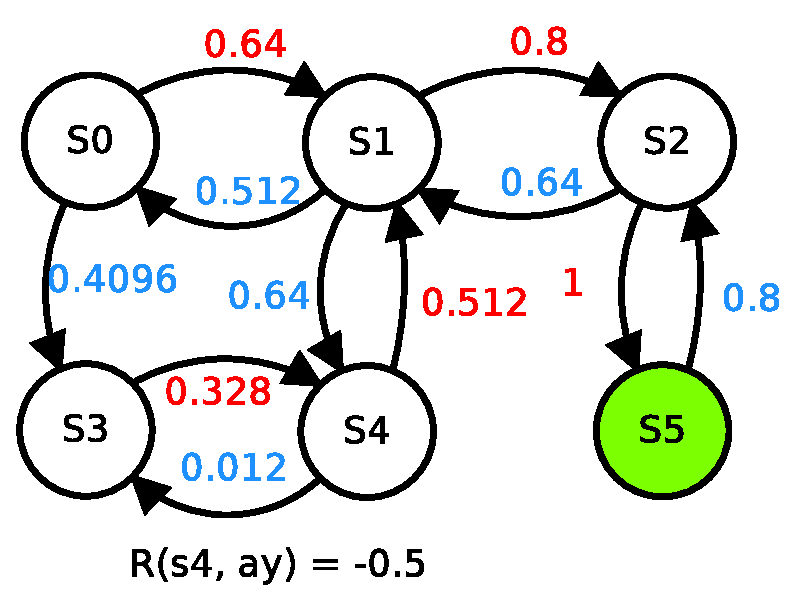
\includegraphics[scale=.6]{../diagrams/q_learning_table_06.eps}
\caption{Konečný stav}
\label{img:q_learning_6}
\end{figure}


\section{Výber akcie}

Pre nájdenie konečných hodnôt funkcie ohodnotení podľa \ref{eq:q_learning_finish}
stačí aby každý prechod mal nenulovú pravdepodobnosť vykonania. Pre ďalšie vyšetrovanie
konania agenta ja daná pravdepodobnosť výberu akcie  ako

\begin{equation}
P(s(n), a(s)) = \frac{e^{kQ(s(n), a(s))}}{ \sum\limits_{i=1}^{C_a}{e^{kQ(s(n), a(i))}} }
\label{eq:action_selection}
\end{equation}

kde \\
$s$ je zvolená akcia \\
$C_a$ je počet akcií \\
$k$ je konštanta a platí $k \geq 0$

agent ktorý vyberá všetky akcie s rovnakou pravdepodobnosťou má teda $k = 0$.
Pre vysoké hodnoty $k$ : $\lim_{k\to\infty}$ bude agent vyberať len najlepšie
dostupné akcie. Pre učenie agenta je teda vhodné zvoliť malé $k$.

Je možné definovať ľubovolné iné možnosti výberu akcie, napr. uprednostňovať menej
často vykonané akcie, prípadne podľa zmeny
$\mid Q_{n}(s(n), a(n)) - Q_{n-1}(s(n), a(n)) \mid$ uprednostňovať prechody s veľkou hodnotou zmeny.


\section{Problémy výpočtu $Q(s, a)$}

Algoritmus je definovaný pre diskrétnu množinu stavov. Ďalej sa predpokladá, že
$s(n) \in \langle -1, 1 \rangle$ a podobne $a(n) \in \langle -1, 1 \rangle$

 Pre počty prvkov
stavového vektora a vektora akcií ($n_s$, $n_a$) je možné definovať
delenie ich hodnôt na diskrétny počet $d_s$ a $d_a$, potom je možné vyjadriť celkový počet
hodnôt $Q(s(n), a(n))$ ako

\begin{equation}
C = {d_s}^{n_s} {d_a}^{n_a}
\label{eq:q_size}
\end{equation}

Samotný počet hodnôt ktoré treba spočítať teda exponenciálne narastná s rastom
počtu prvkov stavového a vektora akcií.

Pre úlohy kde do systému vstupuje mnoho nezávislých vstupov sa stáva implentácia Q(s(n), a(n))
problémom najmä z dôvodov :

\begin{itemize}
\item veľké pamäťové nároky
\item o nenavštívených prechodoch nevie agent povedať nič
\end{itemize}

Vhodným riešením sa ukazuje aproximácia Q-funkcie.
Nech je aproximovaná funkcia označená $Q_n'(s(n), a(n))$ a presné riešenie ako $Q_n(s(n), a(n))$.

Dané sú postuláty o tejto aproximácií
\begin{theorem}{Neobmedzená prenosť aproximácie : }
\label{post:01}
Pre všetky stavy $s(n)$ a akcie $a(n)$ musí platiť
$\mid Q_n(s(n), a(n)) - Q_n'(s(n), a(n)) \mid < \epsilon $. Kde $\epsilon > 0$ a
určuje kvalitu aproximácie. Zlepšením vlastností $Q_n'(s(n), a(n))$ je možné
ľubovolne zmenšovať  $\epsilon$.
\end{theorem}

\begin{theorem}{Lokálna zmena : }
\label{post:02}
Lokálna zmena hodnoty $\delta = \mid Q_n'(s(n), a(n)) - Q_{n-1}'(s(n), a(n)) \mid$ neovplyvní hodnotu funkcie v
inom bode o viac ako $\forall \ s(n') \ \forall a(n'),\ n \neq n' : \delta < \kappa$.
Zmenšovaním hdonoty $\kappa$ sa funkcia stáva menej závislá na okolí bodu $[s(n), a(n)]$.
\end{theorem}

Funkciu $Q(s(n), a(n))$ je možné aproximovať niekoľkými spôsobmi.
Tie najbežnejšie sú

\begin{itemize}
\item tabuľka
\item neurónová sieť
  \begin{itemize}
    \item dopredná neurónová sieť
    \item kohonenova mapa
    \item neurónová sieť bázickych funkcií
  \end{itemize}
\end{itemize}

\section{Tabuľka}

Priamočíarým prístupm je ukladať hodnoty $Q(s(n), a(n))$ do tabuľky. Pre
diskrétnu a konečnú množinu akcií možno tabuľku rozdeliť na viac častí,
čím sa urýchli vyhľadávanie. Počet stavov v reálnych aplikáciach však môže byť
vysoký (vo všeobecnosti tvoria stavy spojitú množinu).

Stav agenta aj vykonaná akcia sú obvykle vektory normované do $\langle -1, 1 \rangle$,
pre implementáciu tabuľky je nutné ich prepočítať na celočíselné indexy

\begin{align}
  I_s(n) = \lceil \sum\limits_{i=1}^{n_s} {\left( d_s\frac{s_i(n) + 1}{2} \right)^i \rceil}  \\
  I_a(n) = \lceil \sum\limits_{i=1}^{n_a} {\left( d_a\frac{a_i(n) + 1}{2} \right)^i \rceil}
\end{align}

kde \\
$I_s(n)$ je index stavu \\
$I_a(n)$ je index akcie \\
$s_i(n)$ je i-ty prvok vektora stavu $s(n)$ \\
$a_i(n)$ je i-ty prvok vektora akcií $a(n)$ \\

Pre diskrétny počet stavov a akcií je možné definovať tabuľkovú interpretáciu ako
$Q^t(I_s(n), I_a(n))$.
Pre $\lim_{d_s\to\infty}$ a $\lim_{d_a\to\infty}$ je možné považovať tabuľku za presné riešenie
pretože spĺňa postuláty \ref{post:01} aj \ref{post:02}.

\section{Dopredná neurónová sieť}

Pre aproximáciu funkcie ohdnotení je možné použiť dobrednú neurónovú sieť ako
univerzálny aproximátor. Podľa Kolmogorovho teorému je možné neurónovú sieť
takto použiť \cite{bib:kolomongorov_01}, \cite{bib:kolomongorov_02} a \cite{bib:kolomongorov_03}.
Samotný teorém však nerieši problém učenia takejto siete. Na učenie siete
existuje niekoľko algoritmov, medzi najčastejšie patria
\cite{bib:backpropagation_00}, \cite{bib:backpropagation_01}, \cite{bib:backpropagation_02} :

\begin{enumerate}
 \item Backpropagation
 \item Genetické algoritmy
 \item Simulované žíhanie
\end{enumerate}

Najpoužívanejší Backpropagation má množstvo problémov, najmä postupný pokles gradientu
v hlbokých neurónových sieťach. Kedy sú vnorené vrstvy prakticky neučené. Ďalší závažný problém
je uviaznutie v lokálnom minime, čo sa autory snažia vyriešiť zavedným zotrvačnosti
do zmeny váh siete. Istým nádejným východiskom sa zdá byť simulované žíhanie \cite{bib:annealing_01}.
Pre problém Q-learning algoritmu je však potrebný prístup ktorý postupne zlepšuje riešenie,
a to je jedine niektorá z gradientových metód.

Samotná dopredná sieť je tvorená niekoľkými prepojenými vrstvami neurónov \ref{img:ffnn}.
Pre popis vrstvy je však vhodné použiť maticový zápis, nakoľko prenos neurónu má
obvykle vo vrstve rovnakú aktivačnú funkciu.

\begin{figure}[!htb]
\center
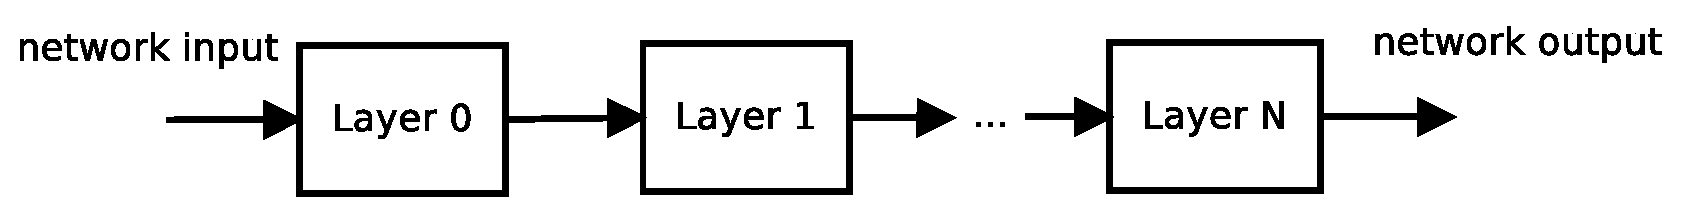
\includegraphics[scale=.6]{../diagrams/neural_layers.eps}
\caption{Dopredná neuronová siet}
\label{img:ffnn}
\end{figure}

Správanie sa jednej vrstvy je možné popísať ako funkciu vstupného vektora,
ktorej výstupom je tiež vektor (počty prvkov týchto vektorov však môžu byť rôzne,
vždy však konečné).
Je daný vstupný vektor

\begin{align}
I(n) = (s(n), a(n))
\label{eq:nn_input_vector}
\end{align}

výstupná hodnota neurónovej siete ako $y_{nn}(n)$ a požadovaná hodnota ako $y_{r}(n)$.

Ďalej je definovaná chyba ako

\begin{align}
e(n) = y_{r}(n) - y_{nn}(n)
\label{eq:nn_error}
\end{align}

Vrstva $l$ doprednej siete je definovaná ako
\begin{align}
y^l(n) &= f^l\left(W^l(n)I^l(n)\right) \nonumber \\
 &= f^l\left(
 \begin{pmatrix}
  w^l_{1,1}(n) & w^l_{1,2}(n) & \cdots & w^l_{1,n'}(n) \\
  w^l_{2,1}(n) & w^l_{2,2}(n) & \cdots & w^l_{2,n'}(n) \\
  \vdots  & \vdots  & \ddots & \vdots  \\
  w^l_{m',1}(n)  & w^l_{m',2}(n)  & \cdots & w^l_{m',n'}(n)
 \end{pmatrix}
 \begin{pmatrix}
  i^l_{1,1}(n) & i^l_{1,2}(n) & \cdots & i^l_{1,n'}(n) \\
 \end{pmatrix}
 \right)
 \label{eq:nn_layer}
\end{align}

kde \\
$n'$ je počet prvkov vstupného vektora \\
$m'$ je počet prvkov výstupného vektora \\
$f(X)$ je aktivačná funkcia \\
$W^l(n)$ je matica váh.

Najčastejšie používané aktivačné funkcie sú sigmoida, hyberbolický tangens , lineárna,
usmerňovač a skoková funkcia. Ich predpisy sú

\begin{align}
y_1(x) &= \frac{1}{1+e^{-x}} \\
y_2(x) &= \frac{e^{x} - e^{-x}}{e^{x} + e^{-x}} \\
y_3(x) &= x \\
y_3(x) &= \left\{
	\begin{array}{ll}
		x  & ak \ x > 0 \\
		0 & inak
	\end{array}
\right. \\
y_4(x) &= \left\{
	\begin{array}{ll}
		1  & ak \ x > 0 \\
		-1 & inak
	\end{array}
\right.
\label{eq:nn_transfer_function}
\end{align}

Ich priebehy sú znázornené na obrázku \ref{img:nn_functions}.

\begin{figure}[!htb]
\center
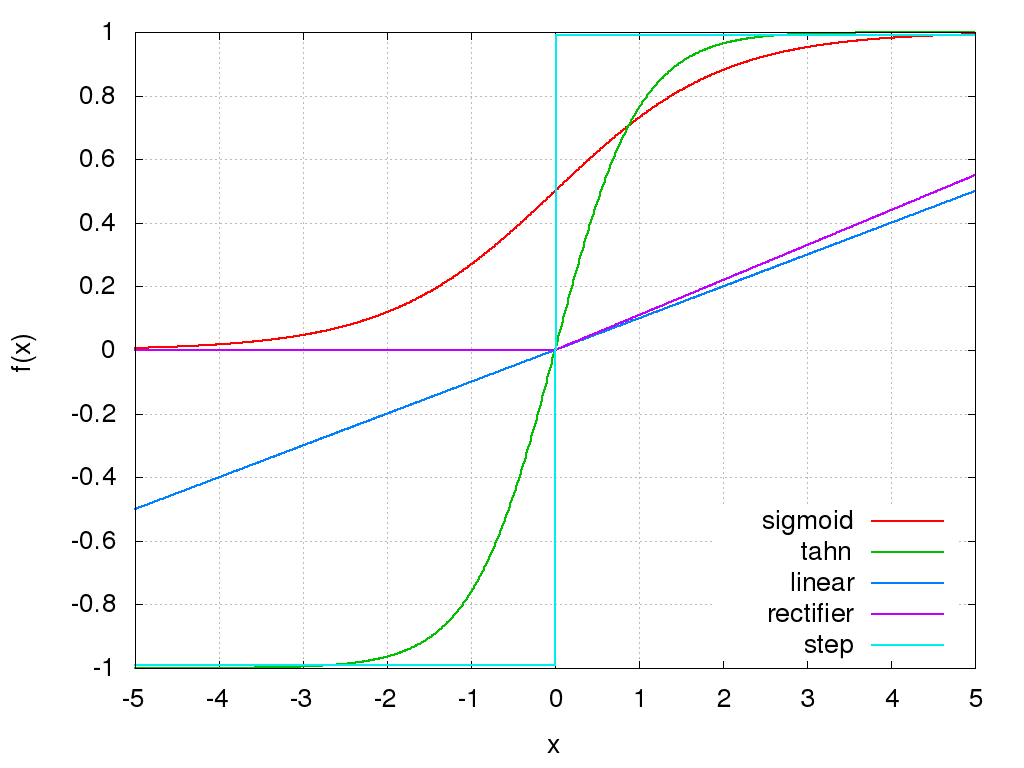
\includegraphics[scale=.4]{../pictures/nn_functions.png}
\caption{Grafické znázornenie priebehov aktivačných funkcií}
\label{img:nn_functions}
\end{figure}

Zoradením niekoľkých vrstiev za sebou, tak že výstup predošlej je vstupom do aktuálnej
vrstvy je možné získať doprednú neurónovu sieť. Takáto sieť je vhodná na riešenie klasifikačných
aj aproximačných problémov.

Dopredná sieť je známa nelokálnosťou učenia : pri trénovaní na podmnožinu množiny
požadovaných výstupov sa mení hodnota aj mimo túto podnmožinu. Sieť teda veľmi
problematicky spĺňa postutlát \ref{post:02}. Dobre však spĺňa postulát \ref{post:01},
vhodnou voľbou počtu vrstiev a počtu neurónov je možné dosiahnúť ľubovolnú
presnosť aproximácie.

\section{Kohonenová neurónová sieť}

Kohonenova neurónová sieť je inšpirovaná rovinnými štruktúrami v mozgovej kôre,
kde výrazne dominujú prepojenia v rámci vrstvy a prepojení medzi vrstvami je
podstatne menej \ref{img:cortical_column}. Napriek týmto rovinatým štruktúram,
mozog bežne spracúva mnohodimenzionálne problémy - vstupm sú podnety s miliónov
receptorov.

\begin{figure}[]
\center
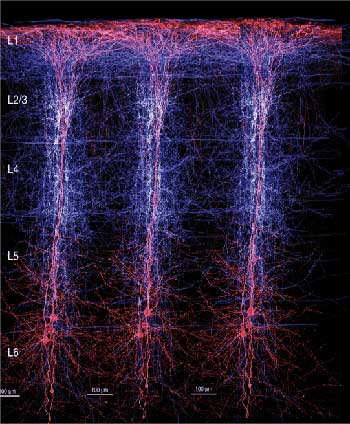
\includegraphics[scale=.4]{../pictures/cortical_column.jpg}
\caption{Neokortexový stĺpec}
\label{img:cortical_column}
\end{figure}

Pôvodný návrh Kohonenovej siete neriešil aproximáciu funkcie, ale klasifikáciu
vstupov do zhlukov. Pričom podobné vstupy patria do rovnakého zhluku. Počet zhlukov
je voliteľný a je rovný počtu použitých neurónov. Takáto sieť sa vie učiť bez
definovania chyby, t.j. nie je potrebné stanoviť do ktorého zhluku dáta patria. Samotné
zhluky sa utvárajú postupne, tak ako sú do siete predkladané dáta.

Každému zhluku je však možné priradiť požadovanú výstupnú hodnotu. Sieť tak môže
pracovať podobne ako tabuľka - vstupné dáta priradí do najbližšieho zhluku a výstupom
je hodnota prisluchújalúca k tomuto zhluku. V tomto prípda už treba stanoviť chybu,
ako rozdiel požadovanej hodnoty a skutočnej hodnoty výstupu siete.
Algoritmus má niekoľko krokov :
\\
Najpr sa spočítajú vzdialenosti od vstupného vektora

\begin{align}
d_j(n) = \sum\limits_{i=1}^{N}{(I_i(n) - w_{ji}(n))^2}
\label{eq:knn_distance}
\end{align}

kde $w(n) \in \mathbb{R}$ je matica váh, na začiatku sa volí náhodná, tak
aby rovnomerne pokrila stavový priestor vstupných veličín (Obvykle sa používa rovnomerné
rozdelenie. Štatistickou analýzou vstupných dát je ale možné určiť iné, vhodnejšie
a urýchliť tak konvergenciu hodnôt váh).

Víťazný neurón $v$ je definovaný ako

\begin{align}
v : \forall j : d_v(n) \leq d_j(n)
\label{eq:knn_winning}
\end{align}

je to neurón ktorý má najmenšiu vzdialenosť od predloženého vstupu.

A pre každý neurón existuje priradená výstupná hodnota $y_j(n) \in \mathbb{R}$, výstupom
siete je teda hodnota priradená výťaznému neurónu $y_{nn}(n) = y_v(n)$.


Učenie siete prebieha v dvoch krokoch

{1) \bf zmena váh $w(n)$ } zmenia sa váhy výťazného neurónu, pretože najlepšie
zodpovedajú požadovaným váham tak že sa priblížia hodnote vstupného vektora

\begin{align}
w_{ji}(n+1) = (1-\eta_1(j))w_{ji}(n) + \eta_1 I_i(n)
\label{eq:knn_w_update}
\end{align}

kde $\eta_1(j) \in (0, 1)$ je krok učenia a závisí od polohy neurónu v sieti.
V najjednoduhšom prípade

\begin{equation}
\eta_1(j) =
\left\{
	\begin{array}{ll}
		\eta  & ak \ j = v \\
		0 & inak
	\end{array}
\right.
\label{eq:knn_func_simple1}
\end{equation}

k zmene váh teda dôjde len pri víťaznom neuróne.
Ďalší často používaný tvar funkcie postupne zmenšuje hodnotu $\eta_1(j)$ podľa
$d_j(n)$ a to ako

\begin{align}
\eta_1(j, n) = \eta e^{-kd_j(n)}
\label{eq:knn_func_simple2}
\end{align}

kde $k \in (0, \infty )$. Krok učenia $\eta_1(j, n)$ je teda premenný a záleží
aj od predloženého vzoru podľa $n$.

Po dostatočnom počte iterácií sa hodnoty váh ustália na hodnotách tak aby rozdelili
množinu vstupných vektorov na lokálne oblasti. Tento stav je znázornený na \ref{img:knn_learning_result}.
Vstupný proces generoval 8 zhlukov dát ktoré sieť klasifikovala použitím 16 neurónov.
Každému neurónu je možne priradiť požadovanú hodnotu výstupu.

{2) \bf upraví sa výstupná hodnota $y_v(n)$}

\begin{align}
y_v(n+1) = y_v(n) + \eta_2 e(n)
\label{eq:knn_y_update}
\end{align}

kde $e(n)$ je chyba podľa \ref{eq:nn_error}.
Takáto Kohonenová sieť má veľmi dobré predpoklady na aprixmáciu funkcie,
ktorá nadobúda málo hodnôt, predkladaním vzorov z blízkosti
jedného zhluku (dáta majú malú vzdialenosť v zmysle \ref{eq:knn_distance} )
sa dá očakávať zmena parametrov len jedného neurónu. Sieť teda dobre spĺňa predpoklady
\ref{post:01},  \ref{post:02}. Počet neurónov však musí narásť do nekonečna.

Je vhodné poznamenať, že výstupná hodnota nemusí byť len číselná hodnota, ale aj funkcia, ktorej vstupom je opäť
$I_i(n)$. Výber výťazného neurónu tak funguje ako výber vhodnej funkcie - prepínač.

\begin{figure}[]
\center
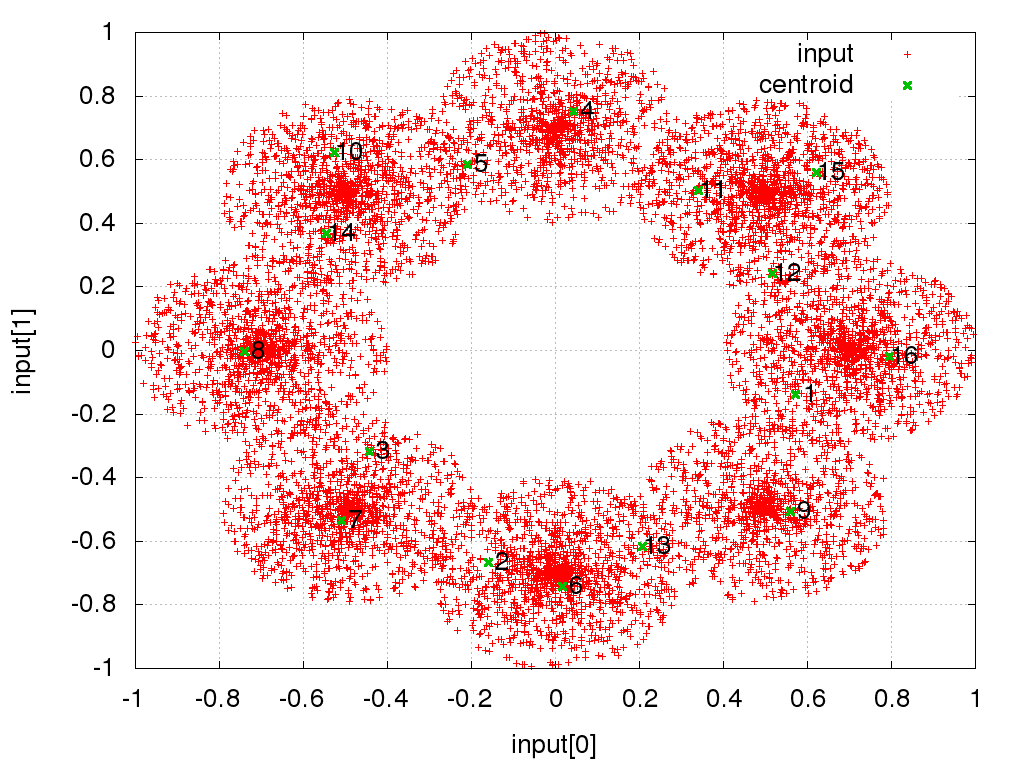
\includegraphics[scale=.4]{../pictures/knn_learing_result.png}
\caption{Znázornenie váhových parametrov w pre dvojrozmerný priestor}
\label{img:knn_learning_result}
\end{figure}

.

\section{Neurónová sieť bázickych funkcií}

Samotný prenos neurónu nemusí byť obmedzený len na množinu funkcií z \ref{eq:nn_transfer_function}.
Vhodnú funkciu je možné zmenou parametrov upraviť do tvaru, aby na zvolený
vstup $I_0(n)$ dosahovala požadovanú hodnotu a postupným zväčšovaním
vzdialenosti $\mid I_0(n) - I_i(n) \mid$ klesala jej hodnota k nule.

Najjednoduhším príkladom takýchto funkcií  je


\begin{equation}
f_j(X(n)) =
\left\{
	\begin{array}{ll}
		k_j  & ak \ X(n) = X_0 \\
		0 & inak
	\end{array}
\right.
\label{eq:bfnn_simple}
\end{equation}

kde $k_j$ je hodnota požadovaná v bode $X_0$. Výstupom siete potom je

\begin{align}
y(X) = \sum\limits_{j=1} f_j(X(n))
\label{eq:bfnn_simple_res}
\end{align}

Z charakteru Q-learning algoritmu majú hodnoty $Q(s(n),a(n))$ charakter aj
postupne klesajúcich hodnôt. Je teda potrebné vybrať iné funkcie.

Nasledujú preto definície funkcií s ktorými boli urobené experimenty.

Dané sú bázické funkcie $f_j^x(\boldmath{s(n), a(n)})$, kde $x$ je typ bázickej funkcie.
Požadovaná hodnota $Q^x(s(n), a(n))$ je potom lineárnou kombináciou týchto funkcií typu $x$.

Z charakteru Q-learning algoritmu \ref{eq:q_learning} je možné určiť požiadavky na
tieto funkcie :

\begin{enumerate}
\item predpis \ref{eq:q_learning} je tvorený klesajúcou exponenciálou - podobný charakter by mala mať aj bázická funkcia
\item existencia jedného globálneho maxima a zmenou parametrov určovať polohu tohto bodu
\item možnosť ľubovolne meniť strmosť funkcie v okolí maxima
\item funkcia by mala byť zhora aj z dola ohraničená
\end{enumerate}

Cieľom je mať možnosť nezávisle nastaviť maximá funkcií do oblastí, ktoré zodpovedajú
nenulovím hodnotám $R(s(n), a(n))$ - bod 2. Ak ohodnotenie spĺňa podmienku najlepšej
možnej akcie v danom stave, dá sa očakávať že bude mať menšiu strmosť, naopak, ak funkcia
popisuje bod kde $R(s(n), a(n))$ dosahuje malé hodnoty (obvykle záporné), bude požadovaná
vysoká strmosť tejto funkcie - obe požiadavky sú zhrnuté v bode 3. Bod 4 umožňuje rozumne
ohraničiť rozsah funkcie.

Niektoré tvary bázických funkcií
\begin{align}
    f_j^1(\boldmath{s(n), a(n)}) &= e^{ -\sum\limits_{i=1}^{n_s}{\beta_{aji}(n)(s_i(n) - \alpha_{aji}(n))^2} }  \\
    f_j^2(\boldmath{s(n), a(n)}) &= \frac{1}{1 + \sum\limits_{i=1}^{n_s}{\beta_{aji}(n)(s_i(n) - \alpha_{aji}(n))^2}}  \\
    f_j^3(\boldmath{s(n), a(n)}) &= e^{ -\sum\limits_{i=1}^{n_s}{\beta_{aji}(n)\mid s_i(n) - \alpha_{aji}(n) \mid} }
    \label{eq:basis_functions_01}
\end{align}

kde \\
$\alpha_{aji}(n) \in \langle -1, 1 \rangle$ určuje polohu maxima funkcie \\
$\beta_{aji}(n) \in (0, \infty)$ určuje strmosť funkcie.

Ich priebeh pre prvé dve je na \ref{img:basis_funcions}.

\begin{figure}[]
\center
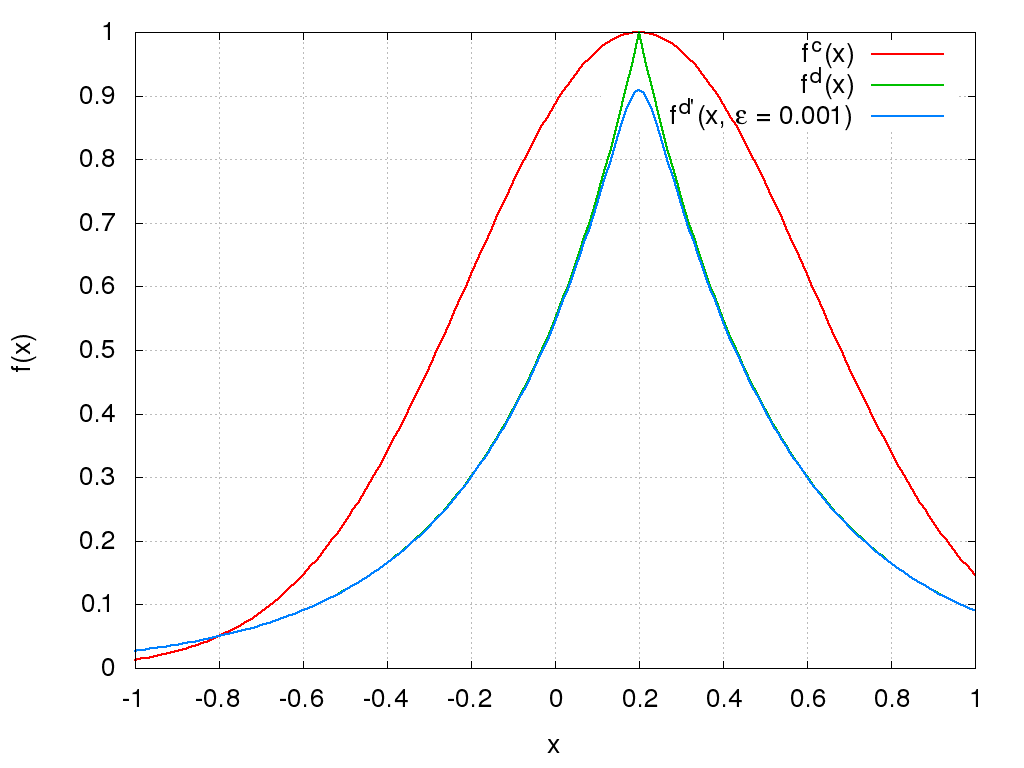
\includegraphics[scale=.4]{../pictures/gaussian_1D.png}
\caption{Znázornenie priebehov bázických fukcií}
\label{img:basis_funcions}
\end{figure}

Pre symetrické prechody medzi stavmi ich možno zjednodušiť na

\begin{align}
f_j^1(\boldmath{s(n), a(n)}) &= e^{ -\beta_{aj} \sum\limits_{i=1}^{n_s}{(s_i(n) - \alpha_{aji})^2} }  \\
f_j^2(\boldmath{s(n), a(n)}) &= \frac{1}{1 + {\beta_{aj} \sum\limits_{i=1}^{n_s}(s_i(n) - \alpha_{aji})^2}}  \\
f_j^3(\boldmath{(n)s, a(n)}) &= e^{ -\beta_{aj} \sum\limits_{i=1}^{n_s}{\mid s_i(n) - \alpha_{aji}(n) \mid} }
\label{eq:basis_functions}
\end{align}

Aproximovaná funkcia ohodnotení pre $l$ bázických funkcií je potom

\begin{align}
Q^x(s(n), a(n)) = \sum\limits_{j=1}^{l} w(n)_j^x f_j^x(\boldmath{s(n), a(n)})
\label{eq:knn_y_update}
\end{align}

kde $w(n)_j^x$ sú váhy bázických funkcií.


Je teda potrebné stanoviť celkovo 3 sady parametrov : $\alpha$ $\beta$ $w$.

\subsection{Určenie parametrov $\alpha$}

Parameter $\alpha$ určuje posunutie maxima funkcie a postupuje sa podobne
ako v prípade \ref{eq:knn_w_update}. Treba zohľadniť fakt, že pre konečný
výsledok je dôležité pokryť všetky oblasti s nenulovým $R(s(n),a(n))$, vrchol
krivky bude ležať nad nad bodom $[s(n),a(n)]$.

Zmena parametrov $\alpha$ prebieha v piatich krokoch.

\begin{itemize}
  \item na začiatku sa zvolia $\alpha_{jia}(n)$ náhodne, ze $\langle -1, 1 \rangle$
  \item spočítajú sa vzdialenosti od predloženého vstupu $d_{ja}(n) = \mid s(n) - \alpha_{ja}(n) \mid$
  \item nájde sa také $ka$ kde pre $\forall{j} : d_{ka}(n) \leq d_{ja}(n)$
  \item spočíta sa krok učenia $\eta'_a(n) = \eta_1 \mid Q_r(s(n), a(n)) \mid$
  \item upravia sa parametre $\alpha_{aki}(n+1) = (1 - \eta')\alpha_{aki}(n) + \eta' s_{i}(n)$
\end{itemize}
kde \\
$Q_r(s(n), a(n))$ je požadovaný výstup \\
$\eta_1$ je konštanta učenia

Krok učenia teda závisí od veľkosti požadovanej hodnoty, tým sa zabezpečí aby maximum
krivky naozaj ležalo nad bodom $[s(n),a(n)]$.

\subsection{Určenie parametrov $\beta$}

Parameter $\beta$ určuje strmosť krivky. Ak boli k dizpozicií naraz všetky
požadované výstupy, bolo by možné spočítat tento parameter z rozptylu.
Požadované hodnoty však prichádzajú postupne, strmosť krivky sa preto upravuje priebežne,
podľa toho či požadovaná hodnota leží nad, alebo pod krivkou.

\begin{itemize}
\item stanoví sa chyba $e(n) = Q_r(s(n), a(n)) - Q(s(n), a(n))$
\item pre každú bázickú funkciu  $\beta_{ja}(n+1)= \beta_{ja}(n) + \eta_2 e(n)w_{ja}(n)$
\item skontroluje sa $\beta_{ja}(n) \in (0, \infty)$
\end{itemize}

kde \\
$Q_r(s(n), a(n))$ je požadovaný výstup \\
$\eta_2$ je konštanta učenia \\


\subsection{Určenie váhových parametrov $w$}

Nakoniec sa gradientovou metódou určia váhové paramete. Pre presné
riešenie by bolo možné použiť metódu nejmenších štvorcov, tá je však pre veľký počet
bázcikých funkcií ťažko vypočítateľná. Zmena parametrov je potom daná nasledujúcim postupom

\begin{itemize}
\item stanoví sa chyba $e(n) = Q_r(s(n), a(n)) - Q(s(n), a(n))$
\item pre každé $w_{ja}$ : $w_{ja}(n+1)= w_{ja}(n) + \eta_3 e(n)y_j(n)$
\item skontroluje sa $w_{ja}(n) \in (-r, r)$
\end{itemize}

kde \\
$\eta_3$ je konštanta učenia \\
$r$ je maximálny rozsah váh \\

\subsection{Hybridný variant}

Ak by funkcia $R(s(n), a(n))$ mala len jednu kladnú hodnotu a ostatné by boli
nulové, aproximáciu $Q(s(n), a(n))$ by veľmi dobre popísala Gaussova krivka \ref{eq:basis_functions}.
Ak by funkcia $R(s(n), a(n))$ mala len záporné hodnoty a ostatné by boli
nulové, funkcia $Q(s(n), a(n))$ by s ohliadnutím na \ref{eq:q_learning} by
si boli rovné. Vo funkcí $Q(s(n), a(n))$ by sa tak objavilo niekoľko záporných
hodnôt, ostro ohraničených.

Vyjdúc z týchto úvah, je možné skombinovať výhody oboch : Gaussova krivka
ktorá dokáže pokryť nenulovými hodnotami celý definyčný obor a funkcie \ref{eq:bfnn_simple}.
Funkcia \ref{eq:bfnn_simple} predstavuje vlastne tabuľku, ktorá nadobúda
nenulové hodnoty vo vybraných bodoch - tvorí tak adaptívnu tabuľku.

Je teda možné skombinovať funkciu \ref{eq:bfnn_simple} s niektorou z \ref{eq:basis_functions},
čo vedie na vzťahy

\begin{align}
P_i(s(n), a(n)) &=
\left\{
	\begin{array}{ll}
		r_{ai}  & if \ s(n) = \alpha^1_i \\
		0 & inak
	\end{array}
\right. \\
  H_j(s(n), a(n)) &= w_{aj} e^{ -\beta_{aj} \sum\limits_{i=1}^{n_s}{(s_i(n) - \alpha^2_{aji})^2 }} \\
  Q(s(n), a(n)) &= \sum\limits_{i=1}^{I} P_i(s(n),a(n)) + \sum\limits_{j=1}^{J} H_j(s(n), a(n))
  \label{eq:peak_hill}
\end{align}

kde \\
$\alpha^1_j$ sú oblasti kde $H_j(s(n))$ nadobúda nenulové hodnoty \\
$\alpha^2_j$ sú oblasti pre ktoré $f_j(\boldmath{s(n), a(n)})$ nadobúda maximum \\
$r_{ai}$ je hodnota okamžitej odmeny $R(s(n))$ v tomto stave \\
$w_{aj}$ je váha a zobovedá veľkosti maxima resp. minima pre fukciu \\
$\beta_{aj}$ je strmosť, a platí $\beta > 0$ \\
$I$ a $J$ sú počty bázických funkcií \\

Označenia $P$ a $H$ vznikli z tvaru funkcií : peak a hill. Funkcia bude na ďalších
grafoch označená ako Gauss + AT : kombinácia Gaussovej krivky a adaptívnej tabuľky.
Mechanizmus učenia zostáva rovnaký ako pre bázické funkcie v predošlej časti. Ukážka
priebehu funkcie pre dve premenné je na obrázku \ref{img:peak_hill_funcion}.
Počet funkcií $P_i(s(n), a(n))$ bol zvolený 30 a počet funkcií $P_i(s(n), a(n))$ 20.
Pre názornosť boli parametre $r_{ai}$ boli zvolené záporné a parametre $\beta_{aj}$ kladné.

\begin{figure}[]
\center
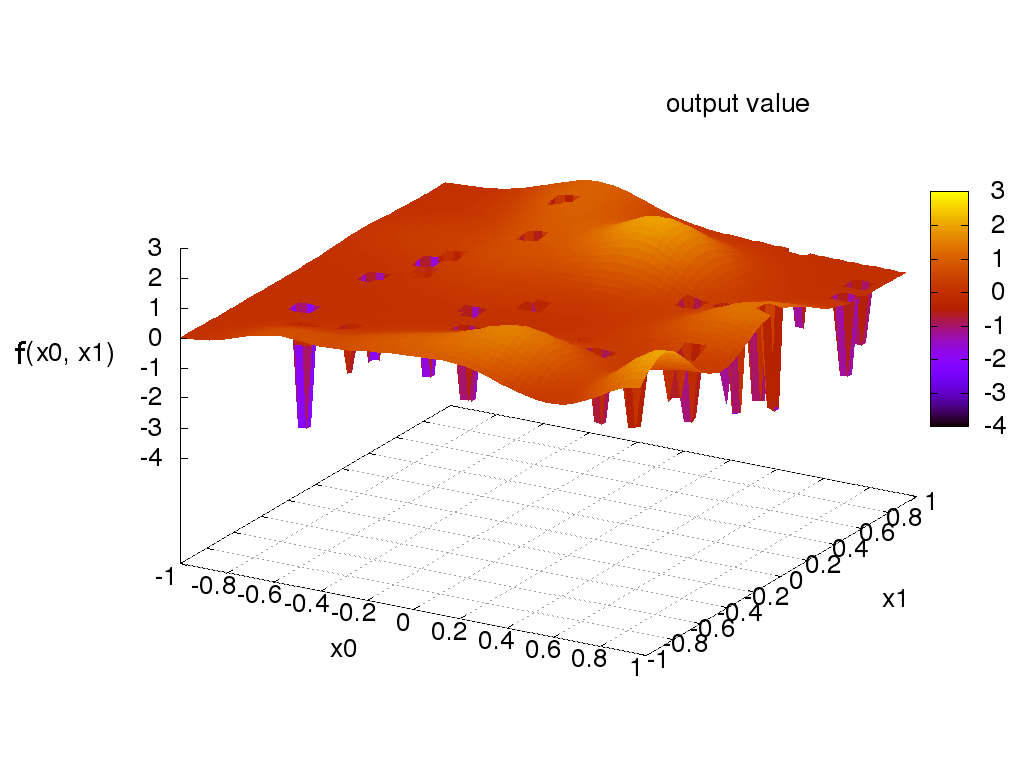
\includegraphics[scale=.5]{../pictures/peak_hill_function.png}
\caption{Znázornenie predmetnej funkcie}
\label{img:peak_hill_funcion}
\end{figure}
